\documentclass[tikz,border=8pt]{standalone}
\usepackage[scaled=0.95]{helvet}
\renewcommand{\familydefault}{\sfdefault}
\usetikzlibrary{arrows.meta}
\definecolor{TEJNavy}{HTML}{1E2B55}
\definecolor{TEJBlue}{HTML}{1769AA}
\begin{document}
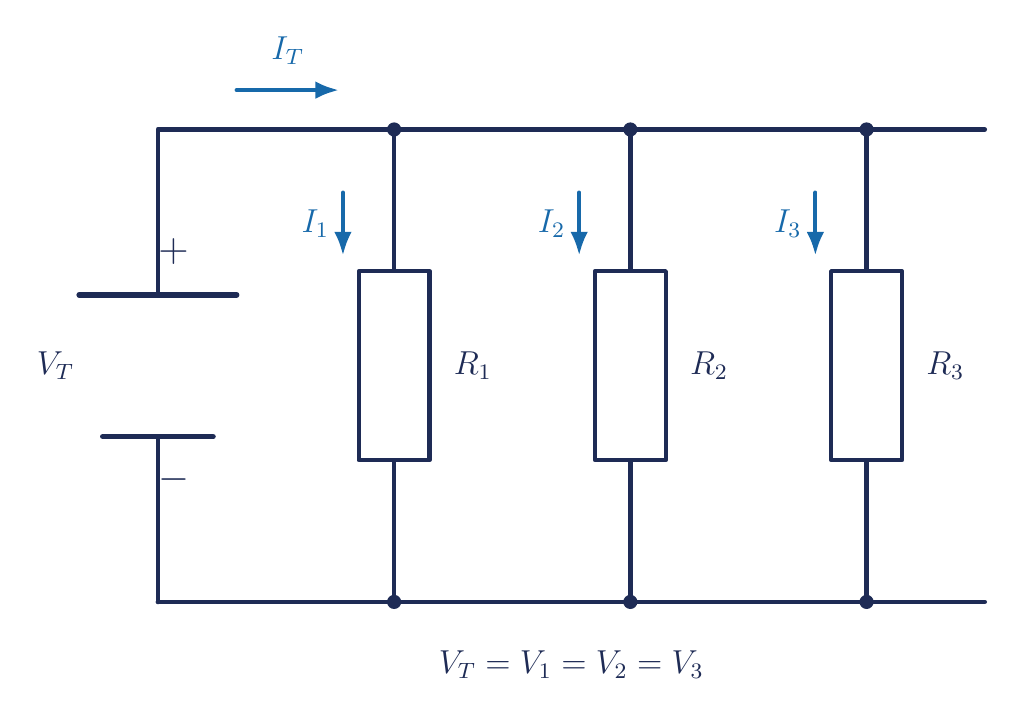
\begin{tikzpicture}[line cap=round,line join=round,font=\sffamily]
  \draw[TEJNavy,line width=1.7pt] (0,0) -- (0,2.1);
  \draw[TEJNavy,line width=1.7pt] (0,3.9) -- (0,6) -- (10.5,6);
  \draw[TEJNavy,line width=1.7pt] (0,0) -- (10.5,0);
  \draw[TEJNavy,line width=2.0pt] (-0.7,2.1) -- (0.7,2.1);
  \draw[TEJNavy,line width=2.0pt] (-1.0,3.9) -- (1.0,3.9);
  \node[font=\bfseries\large,text=TEJNavy] at (-1.3,3.0) {$V_T$};
  \node[font=\bfseries\Large,text=TEJNavy] at (0.2,4.45) {$+$};
  \node[font=\bfseries\Large,text=TEJNavy] at (0.2,1.55) {$-$};
  \foreach \x/\lab in {3/R_1,6/R_2,9/R_3}{
    \draw[TEJNavy,line width=1.7pt] (\x,6) -- (\x,4.2);
    \draw[TEJNavy,line width=1.7pt] (\x,1.8) -- (\x,0);
    \filldraw[fill=white,draw=TEJNavy,line width=1.5pt] (\x-0.45,1.8) rectangle (\x+0.45,4.2);
    \node[font=\bfseries\large,text=TEJNavy] at (\x+1.0,3.0) {$\lab$};
  }
  \draw[-{Latex[length=3mm]},TEJBlue,line width=1.5pt] (1.0,6.5) -- (2.3,6.5);
  \node[font=\bfseries\large,text=TEJBlue] at (1.65,7.0) {$I_T$};
  \foreach \x/\lab in {3/I_1,6/I_2,9/I_3}{
    \draw[-{Latex[length=3mm]},TEJBlue,line width=1.4pt] (\x-0.65,5.2) -- (\x-0.65,4.4);
    \node[font=\bfseries\large,text=TEJBlue] at (\x-1.0,4.8) {$\lab$};
    \fill[TEJNavy] (\x,6) circle (0.09);
    \fill[TEJNavy] (\x,0) circle (0.09);
  }
  \node[font=\bfseries\large,text=TEJNavy] at (5.25,-0.8) {$V_T=V_1=V_2=V_3$};
\end{tikzpicture}
\end{document}
